\documentclass[11pt,a4paper]{article}

\usepackage[margin=1in]{geometry}
\usepackage{graphicx}
\usepackage{booktabs}
\usepackage{amsmath,amssymb}
\usepackage{hyperref}
\usepackage{enumitem}
\usepackage{caption}
\usepackage{subcaption}
\usepackage{natbib}
\usepackage{microtype}

\hypersetup{
  colorlinks=true,
  linkcolor=blue,
  citecolor=blue,
  urlcolor=blue
}

\title{\textbf{Smart-Shield AI: Multimodal Fusion of NLP, Vision, and Tabular Signals for Ontario Highway Safety Routing}}
\author{
  Team 2B --- INFO53883 AI \& ML Capstone\\
  Sheridan College, PAIDA Program\\
  \texttt{[Author names and emails]}
}
\date{Spring 2026}

\begin{document}
\maketitle

\begin{abstract}
We present \emph{Smart-Shield AI}, a proof-of-concept decision-support system that fuses three complementary risk signals---natural-language highway alerts (NLP Brain), road-surface vision estimates (Vision Brain), and environmental/tabular collision history (Environmental Brain)---into a single Safety Score $S \in [0,100]$. The system ranks alternative driving routes on Ontario corridors using free geospatial services (OpenStreetMap, OSRM) and exposes recommendations through an interactive localhost map demo. Trained on Toronto Police Service collision records with supporting UK DfT benchmarks, the pipeline includes Random Forest and optional deep models, SHAP interpretability, and a fairness audit register. We report capstone evaluation metrics and discuss a critical deployment concern raised in peer review, illustrated by a Toronto--Barrie ice-storm demo run ($S=80.6$, advisory 60\,km/h on Hwy~400): \emph{absolute speed advisories} on 100--110\,km/h freeways may increase crash risk via speed differential rather than reduce it. We propose constraint-based, traffic-aware reformulations and trip-level messaging as prerequisites for any operational rollout.
\end{abstract}

\noindent\textbf{Keywords:} highway safety, multimodal fusion, TF-IDF, ResNet18, route choice, Ontario 511, explainable AI

\section{Introduction}
\label{sec:intro}

Ontario's 400-series highways carry high-speed traffic under rapidly changing weather. Official traveller information (511 Ontario) provides textual alerts; collision databases encode historical severity patterns; and onboard or roadside imagery can characterize pavement state. Individually, these modalities leave gaps: text alerts are unstructured, vision models may not generalize across unseen roads, and tabular models lack real-time context.

Smart-Shield AI integrates these streams into a unified Safety Score $S$ and uses it to rank route alternatives in a map-based demo (\url{http://127.0.0.1:5050} in local deployment). The capstone goal is \emph{research and prototyping}, not production traffic management. Nevertheless, peer discussion surfaced an important human-factors question: if the system advises 60\,km/h where the posted limit is 100--110\,km/h and prevailing traffic exceeds the limit, could the recommendation itself create hazard?

This paper describes the architecture, fusion mathematics, evaluation, demo, and---central to responsible reporting---limitations of naïve speed translation from $S$ to km/h.

\section{Related Work}
\label{sec:related}

Traffic crash prediction from historical records is well studied \citep{bokonon2023traffic}. Deep vision (ResNet \citep{he2016resnet}) supports surface-condition classification. Alert text mining aligns with traveller-information systems \citep{ontario511}. Explainability tools such as SHAP \citep{lundberg2017shap} aid auditability in public-sector ML. Our contribution is a \emph{lightweight fusion layer} and open demo stack rather than a new single-modality SOTA predictor.

\section{System Overview}
\label{sec:system}

Figure~\ref{fig:pipeline} summarizes the pipeline implemented in \texttt{notebooks/capstone.ipynb} with modules in \texttt{src/} and deployment artifacts in \texttt{models/}.

\begin{figure}[ht]
  \centering
  \fbox{\parbox{0.92\linewidth}{
    \small
    \textbf{Data:} Toronto TPS collisions + UK DfT benchmark + vision cache\\
    $\downarrow$ preprocess, feature voting (chi$^2$, MI, RF importance)\\
    \textbf{Brains:} NLP (TF-IDF hazard lexicon) \ $|$\ Vision (ResNet18 surface risk $V$) \ $|$\ Tabular RF (collision severity)\\
    $\downarrow$ fusion\\
    \textbf{Safety Score} $S = (w_T T + w_V V + w_E E)\times 100$\\
    $\downarrow$\\
    \textbf{Demo:} Flask API + OSRM routes + Leaflet map (\texttt{demo/api\_server.py})
  }}
  \caption{Smart-Shield pipeline (conceptual).}
  \label{fig:pipeline}
\end{figure}

\subsection{Modalities}

\paragraph{NLP Brain ($T$).}
Ontario 511-style alerts are cleaned and scored with TF-IDF weights over a hazard lexicon (e.g., \emph{black ice}, \emph{blizzard}, \emph{multi-vehicle}). The score $T \in [0,1]$ is normalized against a training corpus of five scenario alerts (TC-1--TC-5).

\paragraph{Vision Brain ($V$).}
A fine-tuned ResNet18 maps road images to surface-risk proxy $V \in [0,1]$. In the map demo, preset weather scenarios map to representative $V$ values when live camera feeds are unavailable.

\paragraph{Environmental / Tabular Brain ($E$).}
An environmental index combines surface, visibility, wind, and temperature risks derived from season, time-of-day, and storm flags. A tuned Random Forest on Toronto collision features provides an auxiliary collision probability (Injury+Fatal).

\subsection{Fusion}
\label{sec:fusion}

Charter weights $(w_T, w_V, w_E) = (0.25, 0.35, 0.40)$ yield
\begin{equation}
  S = \bigl(w_T T + w_V V + w_E E\bigr) \times 100 .
  \label{eq:S}
\end{equation}
Risk tiers follow charter bins: LOW $S \in [0,30]$, MEDIUM $[31,70]$, HIGH $[71,100]$.

The reference implementation maps tiers to speed fractions of posted limit $v_p$ (default 100\,km/h):
\begin{equation}
  v_{\text{rec}} = \round\bigl(v_p \cdot \phi(S)\bigr), \quad
  \phi(S) \in \{1.00,\ 0.80,\ 0.60\}
  \label{eq:speed}
\end{equation}
for LOW, MEDIUM, and HIGH respectively \citep{sheridan_capstone2026}.

\section{Map Demo and Route Ranking}
\label{sec:demo}

The demo geocodes Ontario addresses (Nominatim), fetches up to three OSRM driving routes \citep{osrm,openstreetmap}, and scores each leg with SmartShieldEngine. Routes are sorted by ascending $S$ (lowest = safest pick).

\subsection{Contrasting scenarios: clear vs.\ ice storm}

Table~\ref{tab:toronto-barrie} summarizes two live demo runs on the same origin--destination pair (Toronto $\rightarrow$ Barrie via Highway~400), differing only in the weather preset. Figure~\ref{fig:ice-storm-demo} shows the ice-storm case that triggered peer review.

\begin{table}[ht]
  \centering
  \caption{Toronto--Barrie demo: same route, different weather preset (June 2026 localhost run).}
  \label{tab:toronto-barrie}
  \small
  \begin{tabular}{@{}lccccc@{}}
    \toprule
    Preset & $T$ & $V$ & $E$ & $S$ & $v_{\text{rec}}$ \\
    \midrule
    Clear --- summer highway & 0.00 & 0.08 & 0.17 & 11.3 & 100\,km/h \\
    Ice storm --- QEW rush (pre-fix) & 1.00 & 0.82 & 0.63 & 80.6 & \textbf{60\,km/h} \\
    Ice storm --- QEW rush (post-fix) & 1.00 & 0.82 & 0.63 & 80.6 & \textbf{Avoid travel; $\sim$25\,km/h below flow; clamp 80\,km/h} \\
    \bottomrule
  \end{tabular}
\end{table}

Under clear conditions, $S=11.3$ (LOW tier) and the system recommends the posted 100\,km/h---reasonable for a capstone demo. Under the \emph{Ice storm --- QEW rush} preset (TC-5 alert text, $V=0.82$), fusion yields $S=80.6$ (HIGH tier) and Equation~\eqref{eq:speed} outputs $v_{\text{rec}}=60$\,km/h on a 400-series corridor where posted limits are 100--110\,km/h. The alternate OSRM route scores $S=83.4$ (worse) but receives the same 60\,km/h advisory---correct for ranking, problematic as absolute guidance.

\section{Evaluation (Capstone Scope)}
\label{sec:eval}

Evaluation follows the notebook workflow:
\begin{itemize}[noitemsep]
  \item \textbf{Tabular:} stratified train/test on Toronto severity (Property Damage vs.\ Injury vs.\ Fatal); GridSearchCV for RF/LR; optional DNN.
  \item \textbf{Vision:} hold-out accuracy on cached surface classes.
  \item \textbf{NLP:} hazard-term activation on TC-1--TC-5 scenario alerts.
  \item \textbf{Fusion dashboard:} scenario table comparing $T$, $V$, $E$, and $S$.
  \item \textbf{Explainability:} SHAP on tuned RF features.
  \item \textbf{Ethics:} fairness audit register (Section 7 of notebook).
\end{itemize}

Full numeric tables should be copied from the latest notebook run into an appendix before journal submission.

\section{Discussion: Speed Advisory Critique}
\label{sec:speed-critique}

During peer review, a fellow researcher asked:
\emph{``If AI advises 60\,km/h on a highway currently operating at 100--110\,km/h, would that not cause an accident?''}

Figure~\ref{fig:ice-storm-demo} instantiates this concern with a reproducible capstone example.

\begin{figure}[ht]
  \centering
  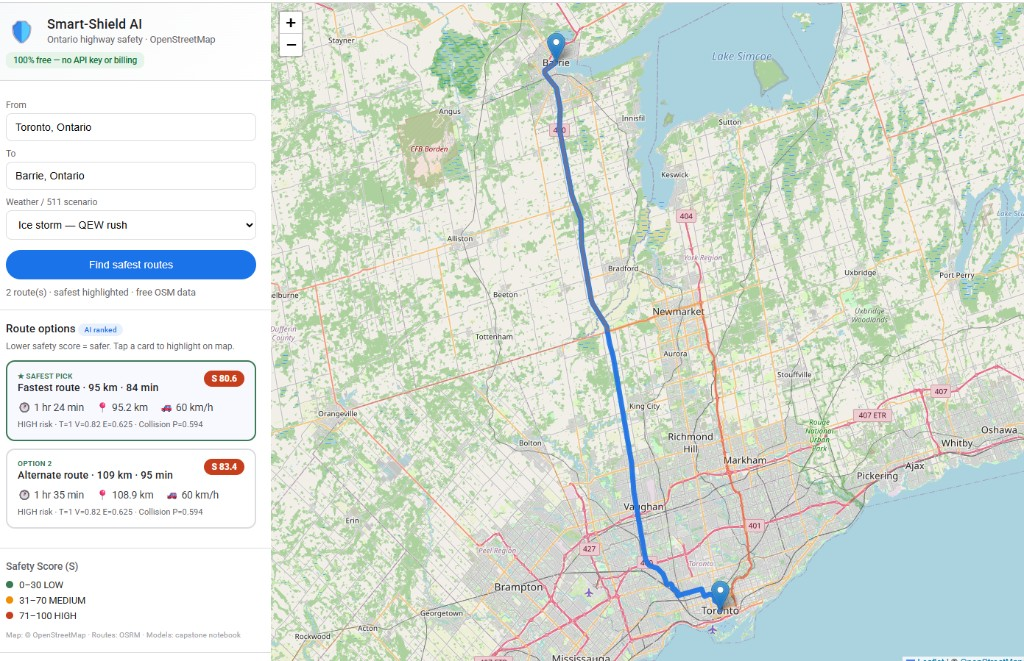
\includegraphics[width=\linewidth]{figures/ice_storm_toronto_barrie_demo.png}
  \caption{Smart-Shield demo: Toronto $\rightarrow$ Barrie, \emph{Ice storm --- QEW rush} preset. Safest route (Hwy~400): $S=80.6$ (HIGH), recommended 60\,km/h, $T{=}1$, $V{=}0.82$, $E{=}0.625$, Collision $P{=}0.594$. Screenshot from localhost deployment (\url{http://127.0.0.1:5050}).}
  \label{fig:ice-storm-demo}
\end{figure}

\subsection{Worked example: why $S=80.6$ and 60\,km/h appear}
\label{sec:worked-example}

For the ice-storm preset, the demo injects TC-5 alert text (freezing rain, black ice, multi-vehicle collision), setting $T=1$ after hazard-term saturation. The vision preset sets $V=0.82$. With \texttt{is\_winter\_storm=True} but a non-winter calendar month in the demo run, the environmental index was $E=0.625$ (surface and wind at storm levels; temperature term reduced). Base fusion from Equation~\eqref{eq:S}:
\begin{align*}
  S_{\text{base}} &= (0.25 \times 1.00 + 0.35 \times 0.82 + 0.40 \times 0.625) \times 100 \\
                  &\approx 78.7 .
\end{align*}
Route-level adjustments in \texttt{demo/inference.py} add up to 6\,points for distance ($\min(6, 0.02 \times 95.2)$), yielding $S \approx 80.6$ for the fastest leg. Because $S \geq 71$, tier HIGH applies. \textbf{Pre-fix:} $v_{\text{rec}} = \round(100 \times 0.60) = 60$\,km/h. \textbf{Post-fix (SS-AUDIT-2026-001):} \texttt{build\_operational\_advisory()} separates ranking from operations---primary message \emph{avoid/postpone travel}; relative guidance to reduce speed by $\sim$25\,km/h below assumed prevailing flow ($\sim$105\,km/h); clamped absolute floor 80\,km/h on 400-series demo defaults (naive 60\,km/h retained for audit only).

The UI correctly communicates \textbf{high environmental risk}. The open question is whether \textbf{60\,km/h in a live travel lane} is the right \emph{operational} response when surrounding traffic on Hwy~400 may still be flowing at 80--100+\,km/h during the early phase of a storm---or whether the primary message should be \emph{do not travel} or \emph{exit highway}.

This is a substantive concern, not a cosmetic UI issue. Under Equation~\eqref{eq:speed}, HIGH tier ($S \geq 71$) implies $v_{\text{rec}} = 60$\,km/h when $v_p = 100$\,km/h. On Ontario freeways, posted limits are often 100--110\,km/h and prevailing speeds frequently exceed posted limits in good conditions. A 40--50\,km/h speed differential between advised drivers and the main traffic stream increases:
\begin{enumerate}[noitemsep]
  \item \textbf{Rear-end and lane-change conflicts} (closing speed from following traffic);
  \item \textbf{Side-swipe risk} when slower vehicles occupy travel lanes rather than shoulders;
  \item \textbf{Compliance friction} (drivers ignoring advice) or \textbf{over-compliance} (dangerous slowing in live lanes);
  \item \textbf{Legal ambiguity} relative to minimum-speed expectations on controlled-access highways.
\end{enumerate}

Thus, Equation~\eqref{eq:speed} is acceptable for \emph{capstone demonstration} but \textbf{not} for operational deployment without reformulation. Audit SS-AUDIT-2026-001 implemented trip-level messaging, relative speed text, and an 80\,km/h freeway floor in \texttt{src/safety\_score.py} and the localhost demo. Full tracking: \texttt{improvements/speed-advisory-audit/}.

\subsection{Recommended Improvements}
\label{sec:improvements}

We group mitigations by system layer:

\paragraph{1. Constraint-based advisories (immediate).}
Replace absolute $v_{\text{rec}}$ with bounded relative guidance:
\begin{equation}
  v_{\text{rec}} = \min\!\Bigl(v_p,\ \max\bigl(v_{\min}^{\text{safe}},\ v_p \cdot \phi(S)\bigr)\Bigr)
\end{equation}
where $v_{\min}^{\text{safe}}$ is derived from posted minimum-speed rules and a \emph{traffic-aware floor} (e.g., 85th percentile speed from probe data minus a safety margin). Message users in \textbf{relative} terms: ``reduce speed by 15--20\,km/h below prevailing traffic'' rather than ``drive 60\,km/h.''

\paragraph{2. Trip-level vs.\ lane-level messaging.}
For HIGH $S$, prioritize:
\begin{itemize}[noitemsep]
  \item \textbf{Avoid travel} / delay trip;
  \item \textbf{Use alternate route} (already supported by multi-route ranking);
  \item \textbf{Exit and wait} at service centre;
  \item Only if continuing: \textbf{right lane, hazard lights, match truck pace}---not arbitrary absolute caps in left lanes.
\end{itemize}

\paragraph{3. Traffic and infrastructure context.}
Integrate 511 Ontario live feeds, loop-detector or probe speeds, construction zones, and lane closures. Fusion should condition on \emph{current} traffic speed distribution, not static $v_p$.

\paragraph{4. Separate risk dimensions.}
Decouple \emph{collision risk} (historical/tabular), \emph{environmental hazard} ($E$, $V$), and \emph{operational feasibility} (speed variance penalty). Add explicit penalty term $S_{\Delta v}$ when $|v_{\text{rec}} - \bar{v}_{\text{traffic}}|$ exceeds a threshold.

\paragraph{5. Calibration and validation.}
Validate advisories with microsimulation (SUMO/VISSIM) or naturalistic driving datasets; report not only crash probability but \emph{surrogate safety measures} (time-to-collision, deceleration rate). Engage human-factors review aligned with MTO practices.

\paragraph{6. Model calibration note.}
Demo outputs may show high collision probability ($P \approx 0.59$) even under LOW $S$ when RF outputs are marginal---suggesting miscalibration between tier labels and probability display. Platt scaling or isotonic calibration on held-out data should precede user-facing $P$.

\paragraph{7. Governance.}
Position Smart-Shield as \textbf{decision support}, not autonomous control; require human confirmation; log overrides for audit.

\section{Limitations}
\label{sec:limits}

\begin{itemize}[noitemsep]
  \item Small NLP corpus (five scenario alerts); TF-IDF does not capture semantic novelty.
  \item Vision presets in demo substitute for live cameras.
  \item Toronto-trained tabular model may not transfer to all Ontario corridors.
  \item Route geometry risk (curvature, grade) not yet in $S$.
  \item Speed recommendation formula (Eq.~\eqref{eq:speed}) ignores traffic-flow coupling (Section~\ref{sec:speed-critique}).
  \item No prospective field trial or IRB-approved user study.
\end{itemize}

\section{Future Work}
\label{sec:future}

\subsection{Technical extensions}
Priority model and demo extensions: (i)~\textbf{traffic-aware speed floors and relative advisories}---partially implemented in audit SS-AUDIT-2026-001 via \texttt{build\_operational\_advisory()}; (ii)~expanded 511 NLP corpus with transformer embeddings; (iii)~live vision via MTO camera APIs; (iv)~graph-based route features from OSM; (v)~multi-objective ranking ($S$, time, distance, cost); (vi)~calibration and fairness testing on regional subgroups; (vii)~optional EV fast-charging layer along route polylines (Open Charge Map / OSM); (viii)~partnership pathway with transportation agencies for pilot design.

\subsection{Deployment: route planning and ERP integration}
Beyond the localhost demo, Smart-Shield is architected as a \textbf{safety scoring microservice} that ERP and TMS platforms can call before dispatch. Typical flow: sales or transport orders in ERP $\rightarrow$ route alternatives from OSRM or commercial engines $\rightarrow$ Smart-Shield ranks legs by $S$ and returns \texttt{operational\_guidance} $\rightarrow$ dispatcher confirms or overrides (logged) $\rightarrow$ navigation executes turn-by-turn.

\paragraph{Individual use cases.}
Daily commuters comparing Toronto--Barrie alternates under ice-storm alerts; EV drivers combining safety ranking with charger proximity (future layer); rideshare and gig workers screening HIGH-tier corridors before accepting trips.

\paragraph{Business use cases.}
Fleet logistics and LTL line-haul (crew safety, liability audit trail); last-mile delivery (delay high-$S$ manifests); field service dispatch (Dynamics, Salesforce Field Service); school transportation route review; construction oversize corridor selection; insurance/telematics analytics exporting tier history per \texttt{trip\_id}.

\paragraph{ERP touchpoints.}
Order-to-cash delivery promises; TMS dispatch boards; HR shift rules blocking \texttt{AVOID\_TRAVEL} without override; finance chargebacks for weather delays; analytics warehouses storing immutable safety audit rows. Integration patterns include synchronous REST (\texttt{POST /api/score-routes}), event-driven scoring (Kafka / Azure Service Bus), and embedded Fiori or Dynamics widgets. Full use-case and ERP mapping: \texttt{docs/ROUTE-PLANNING-USE-CASES-AND-ERP.md}.

Governance requirements for production: human-in-the-loop confirmation, override logging, calibrated collision $P$, and explicit non-claim of MTO operational authority.

\section{Conclusion}
\label{sec:conclusion}

Smart-Shield AI demonstrates that fusing alert text, vision proxies, and collision history into a single Safety Score enables interpretable, multimodal route ranking in an open demo stack. The peer critique on 60\,km/h vs.\ 100--110\,km/h traffic underscores that \emph{risk minimization in a model is not equivalent to safe operational guidance}. Publishable next steps focus on traffic-aware constraints, trip-level messaging, and validated calibration---before any claim of accident reduction on live highways.

\section*{Acknowledgments}
Sheridan College INFO53883 instructors and capstone reviewers; OpenStreetMap and OSRM communities.

\bibliographystyle{plainnat}
\bibliography{references}

\appendix
\section{Repository Layout (Reproducibility)}
\label{app:repo}

\begin{tabular}{@{}ll@{}}
\toprule
Path & Role \\
\midrule
\texttt{notebooks/capstone.ipynb} & Training and evaluation \\
\texttt{src/nlp\_brain.py} & NLP Brain \\
\texttt{src/vision\_brain.py} & Vision Brain \\
\texttt{src/safety\_score.py} & Fusion and speed tiers \\
\texttt{models/} & Saved \texttt{.joblib} / \texttt{.pt} artifacts \\
\texttt{demo/api\_server.py} & Localhost map server (port 5050) \\
\bottomrule
\end{tabular}

\section{Demo Run Commands}
\label{app:demo}

\begin{verbatim}
conda activate ai_work_final
cd .../INFO53883 - AI & ML Capstone Project/demo
pip install -r requirements-demo.txt
python api_server.py
# Browser: http://127.0.0.1:5050
\end{verbatim}

\section{Post-Fix Speed Advisory (SS-AUDIT-2026-001)}
\label{app:postfix}

After peer review, \texttt{build\_operational\_advisory()} returns fields separate from Safety Score $S$:

\begin{tabular}{@{}ll@{}}
\toprule
Field & Ice storm example ($S=80.6$) \\
\midrule
\texttt{operational\_guidance} & \texttt{AVOID\_TRAVEL} \\
\texttt{operational\_message} & Consider postponing this trip \\
\texttt{naive\_recommended\_speed\_kmh} & 60 (legacy $\phi$ formula) \\
\texttt{recommended\_speed\_kmh} & 80 (400-series clamp) \\
\texttt{relative\_speed\_text} & Reduce $\sim$25\,km/h below $\sim$105\,km/h flow \\
\bottomrule
\end{tabular}

Ranking ($S$, tier colours) is unchanged; only user-facing guidance differs from the pre-fix screenshot.

\section{Business Value \& ERP Integration (One-Page Summary)}
\label{app:business}

This appendix summarizes deployment value for capstone reviewers and industry stakeholders. Full detail: \texttt{docs/ROUTE-PLANNING-USE-CASES-AND-ERP.md}.

\subsection*{Value proposition}
Smart-Shield AI is a \textbf{safety scoring microservice} for route choice: fuse 511-style alerts (NLP), road-surface vision proxies, and collision-history signals into Safety Score $S \in [0,100]$, then return \textbf{operational guidance} (e.g.\ postpone travel, relative speed advice) \emph{separate} from ranking. It complements---does not replace---navigation engines (OSRM, Google) and ERP/TMS dispatch workflows.

\subsection*{Individual use cases}
\begin{itemize}[noitemsep]
  \item \textbf{Commuters:} Compare Toronto--Barrie alternates under ice-storm alerts; HIGH-tier banner before departure.
  \item \textbf{EV drivers:} Safety-ranked routes plus future fast-charger proximity layer.
  \item \textbf{Rideshare / gig:} Screen HIGH-$S$ corridors before accepting trips.
  \item \textbf{Families:} ``Safest pick'' among alternates with interpretable $T$, $V$, $E$ breakdown.
\end{itemize}

\subsection*{Business use cases}
\begin{itemize}[noitemsep]
  \item \textbf{Fleet / LTL:} Rank line-haul alternates; audit trail for duty-of-care and liability.
  \item \textbf{Last-mile:} Delay or reroute manifests when $S \geq 71$ before lock.
  \item \textbf{Field service:} Score technician routes (Dynamics, Salesforce Field Service).
  \item \textbf{Insurance / telematics:} Export tier history per \texttt{trip\_id} for analytics.
  \item \textbf{Public sector:} Winter-ops decision support (non-operational prototype).
\end{itemize}

\subsection*{ERP integration flow}
\begin{center}
\small
ERP order $\rightarrow$ TMS route options $\rightarrow$ \textbf{Smart-Shield scores legs} $\rightarrow$ dispatcher confirms/overrides (logged) $\rightarrow$ navigation executes
\end{center}

\noindent\textbf{Touchpoints:} order-to-cash delivery promises; dispatch boards; HR rules blocking \texttt{AVOID\_TRAVEL}; finance weather-delay codes; analytics warehouses (Power BI, SAP BW, Snowflake).

\noindent\textbf{Patterns:} REST \texttt{POST /api/score-routes}; event-driven scoring (Kafka / Service Bus); embedded Fiori or Dynamics widgets.

\subsection*{Governance (production prerequisites)}
Human-in-the-loop confirmation; immutable override logs; calibrated collision probability; explicit disclaimer---research prototype, not MTO operational authority.

\vspace{0.5em}
\noindent\textbf{Tagline:} \emph{Multimodal safety scoring for route choice---for commuters today and ERP/TMS dispatch tomorrow.}

\end{document}
